Because of the decision to recreate the game from scratch, this sprint has been more like a pregame from SCRUM, and the actual product is therefore minimal.
The framework that was suggested in \stefan{ref} has been used to recreate a minimal working example of the game.
The result can be seen on \ref{product-sprint1}.

The car drives from left to right and is controlled by the volume of the player's voice. 
Loud sounds will make the car drive to its left while quiet sounds make it drive to its right.
Only sounds over a certain threshold makes the car move, meaning that no sound causes the car to drive straight forward.

The squares in the right side of the screen represent garages, and the color represents its state. 
A green garage is open, a yellow garage is closing while a red garage is closed.
It is possible to drive into a green garage which will then turn yellow for a short amount of time and then turning red.
If the car drives into a red garage it 'crashes', resetting its position to the starting position in left of the map vertically in the middle of the screen.

The purple squares represent obstacles that have to be avoided. 
If the car drives into one of these it 'crashes' and is being reset.


\begin{figure}
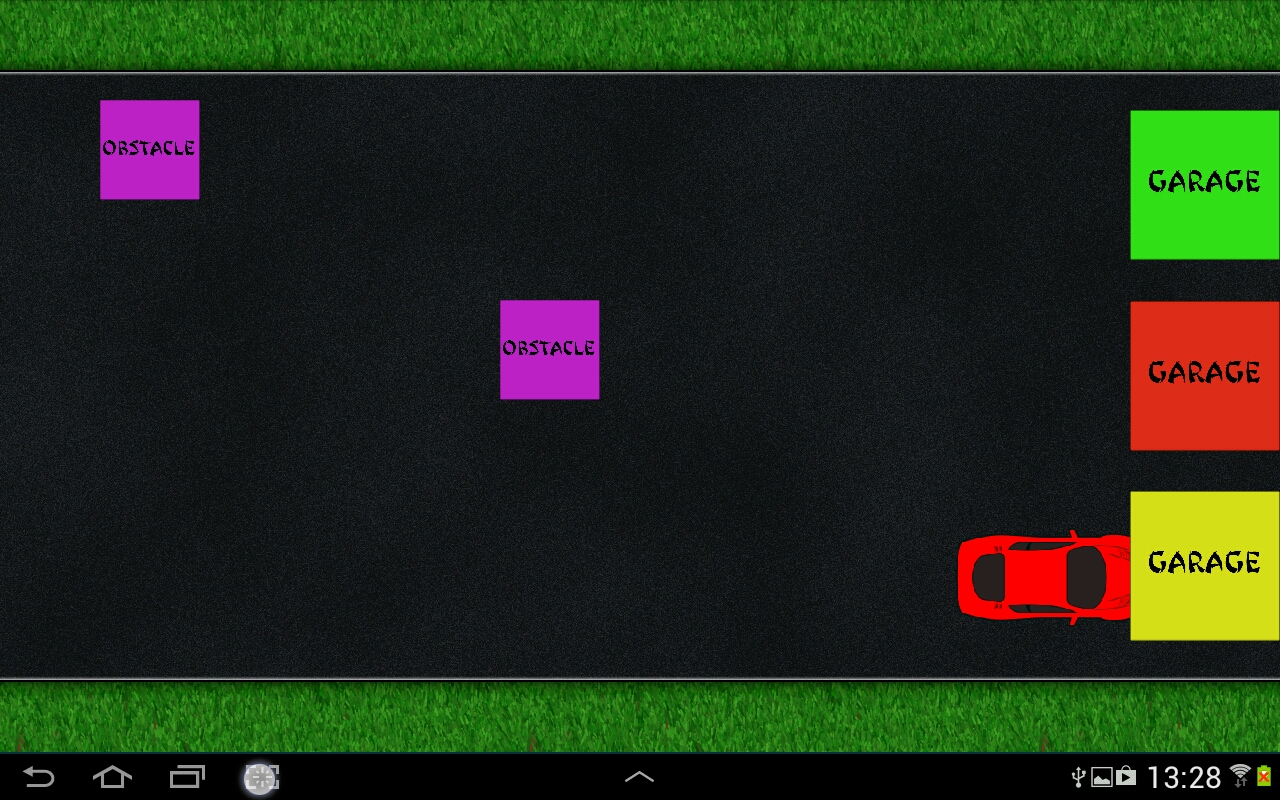
\includegraphics[width=\textwidth]{product}
\caption{The product after sprint 1}
\label{product-sprint1}
\end{figure}